\documentclass[tikz,border=4pt]{standalone}
% Shared visual grammar: role fills, dark connectors, and 7-point typography.
% Build each standalone figure from this directory. No external images required.
\pdfinfoomitdate=1
\pdftrailerid{}
\usepackage[T1]{fontenc}
\usepackage{helvet}
\renewcommand{\familydefault}{\sfdefault}
\usepackage{amsmath,amssymb}
\hyphenpenalty=10000
\exhyphenpenalty=10000
\usetikzlibrary{arrows.meta,calc,fit,positioning,decorations.pathreplacing,backgrounds}
\definecolor{ink}{HTML}{172B3A}
\definecolor{muted}{HTML}{586D85}
\definecolor{datafill}{HTML}{F1F5F9}
\definecolor{dataline}{HTML}{62748E}
\definecolor{modelfill}{HTML}{E5E9FF}
\definecolor{modelline}{HTML}{7887C7}
\definecolor{llmfill}{HTML}{FFE4E8}
\definecolor{llmline}{HTML}{E68494}
\definecolor{truthfill}{HTML}{D0FAE5}
\definecolor{truthline}{HTML}{35A782}
\newcommand{\seven}{\fontsize{7}{8.5}\selectfont}
\tikzset{
 every node/.append style={font=\seven,text=ink,align=center},
 box/.style={draw=dataline,fill=white,rounded corners=3pt,line width=.65pt,inner sep=5pt,minimum height=8mm},
 data/.style={box,fill=datafill},
 model/.style={box,draw=modelline,fill=modelfill},
 llm/.style={box,draw=llmline,fill=llmfill},
 truth/.style={box,draw=truthline,fill=truthfill},
 title/.style={font=\seven\bfseries,inner sep=1pt},
 word/.style={text=muted,inner sep=1pt,align=center},
 label/.style={fill=white,inner xsep=2pt,inner ysep=1pt,text=muted},
 flow/.style={-{Stealth[length=2.4mm,width=1.9mm]},draw=ink,line width=1.2pt,shorten >=1.5pt},
 branch/.style={-{Stealth[length=2mm,width=1.6mm]},draw=ink,line width=.9pt,shorten >=1pt},
 route/.style={draw=ink,line width=1.2pt},
 update/.style={-{Stealth[length=2.2mm,width=1.7mm]},draw=modelline,line width=1pt,dash pattern=on 3pt off 2pt,shorten >=1.5pt},
 boundary/.style={draw=dataline,dash pattern=on 3pt off 2pt,rounded corners=3pt,line width=.6pt},
 chip/.style={minimum height=4mm,inner xsep=3pt,inner ysep=1.5pt,rounded corners=2pt},
}
% Optional role key. Anchor at the center of an uncluttered final row.
\newcommand{\rolekey}[2]{
 \node[word,anchor=east] at (#1-6.6,#2) {\textit{Key}};
 \node[data,chip] at (#1-5.2,#2) {records / data};
 \node[model,chip] at (#1-1.9,#2) {learned model / policy};
 \node[llm,chip] at (#1+1.65,#2) {LLM signal};
 \node[truth,chip] at (#1+4.95,#2) {labels / evaluation};
}

\begin{document}
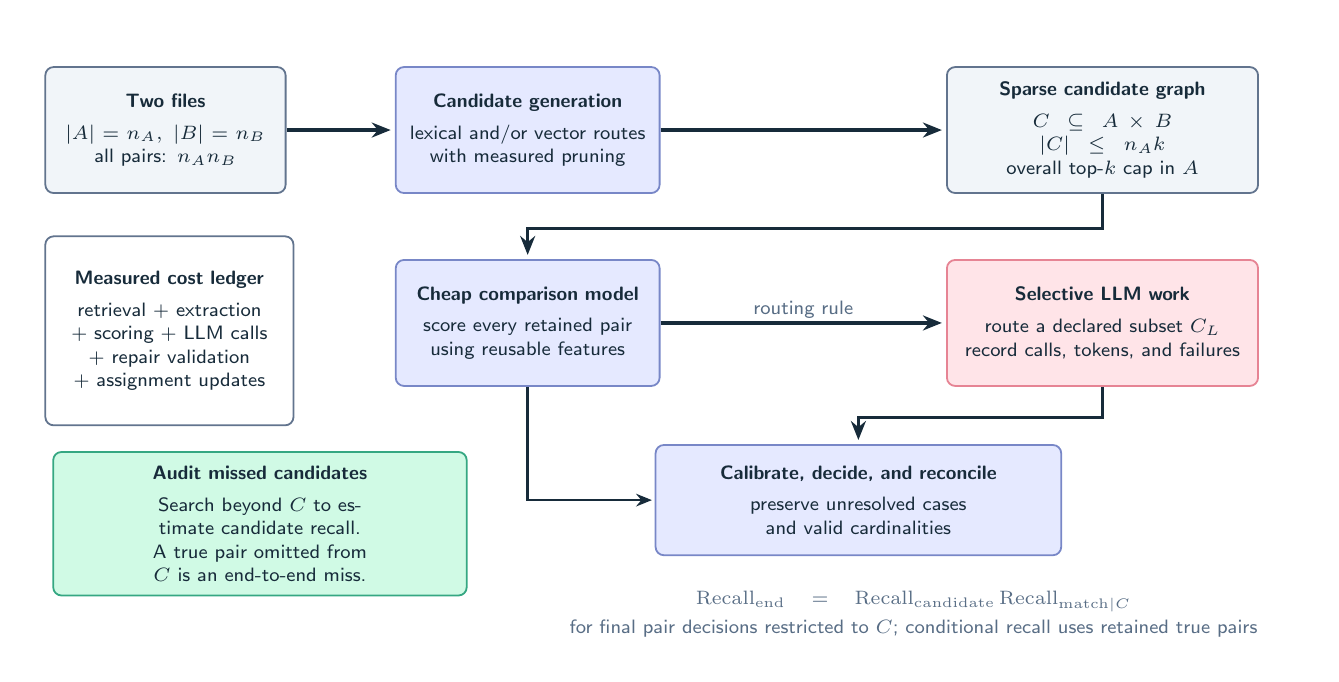
\begin{tikzpicture}

\useasboundingbox (-.2,.3) rectangle (16.1,-7.65);
\node[data,text width=27mm,minimum height=16mm] (files) at (1.55,-1.0) {\textbf{Two files}\\[3pt]$|A|=n_A,\ |B|=n_B$\\all pairs: $n_A n_B$};
\node[model,text width=30mm,minimum height=16mm] (retrieval) at (6.15,-1.0) {\textbf{Candidate generation}\\[3pt]lexical and/or vector routes\\with measured pruning};
\node[data,text width=36mm,minimum height=16mm] (graph) at (13.45,-1.0) {\textbf{Sparse candidate graph}\\[3pt]$C\subseteq A\times B$\\$|C|\leq n_A k$\\overall top-$k$ cap in $A$};
\draw[flow] (files) -- (retrieval); \draw[flow] (retrieval) -- (graph);
\node[model,text width=30mm,minimum height=16mm] (cheap) at (6.15,-3.45) {\textbf{Cheap comparison model}\\[3pt]score every retained pair\\using reusable features};
\node[llm,text width=36mm,minimum height=16mm] (llm) at (13.45,-3.45) {\textbf{Selective LLM work}\\[3pt]route a declared subset $C_L$\\record calls, tokens, and failures};
\draw[flow] (graph.south) -- (13.45,-2.25) -- (6.15,-2.25) -- (cheap.north);
\draw[flow] (cheap) -- node[label,above] {routing rule} (llm);
\node[box,text width=28mm,minimum height=24mm] (cost) at (1.6,-3.55) {\textbf{Measured cost ledger}\\[3pt]retrieval + extraction\\+ scoring + LLM calls\\+ repair validation\\+ assignment updates};
\node[model,text width=48mm,minimum height=14mm] (decision) at (10.35,-5.7) {\textbf{Calibrate, decide, and reconcile}\\[3pt]preserve unresolved cases and valid cardinalities};
\draw[flow] (llm.south) -- (13.45,-4.65) -| (decision.north);
\draw[branch] (cheap.south) -- (6.15,-5.7) -- (decision.west);
\node[truth,text width=49mm,minimum height=18mm] at (2.75,-6.0) {\textbf{Audit missed candidates}\\[3pt]Search beyond $C$ to estimate candidate recall.\\A true pair omitted from $C$ is an end-to-end miss.};
\node[word,text width=88mm] at (11.05,-7.15) {$\mathrm{Recall}_{\mathrm{end}}=\mathrm{Recall}_{\mathrm{candidate}}\,\mathrm{Recall}_{\mathrm{match}\mid C}$\\[2pt]for final pair decisions restricted to $C$; conditional recall uses retained true pairs};

\end{tikzpicture}
\end{document}
